Two main experiments have been conducted; the first experiment involves applying the aforementioned machine learning methods on the feature extracted vector. The second experiment involves applying deep learning practices on the raw image data. 

\subsection*{Experiment 1: Machine Learning}
The machine learning experiments are implemented in Python 3 using the SciKit Learn library, except the Neural Network that are implemented in Keras using Tensorflow backend. \\

All classifiers have been run on the FIN-Benthic dataset and on the FIN-Benthic concatenated dataset using Grid Search and CV to find the best hyperparameters, except the neural networks. As grid search has been used to find the best set of parameters for each of the classifiers and on the different datasets, it has not given the same results for best hyperparameter settings. Only the best performing setting of hyperparameters for each classifier are presented in this paper.

\begin{figure}[H]
    \centering
    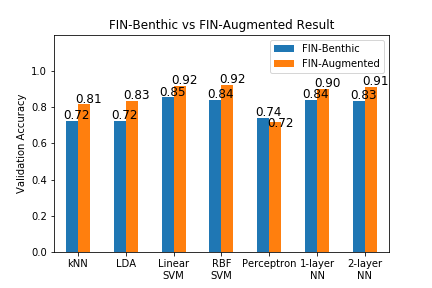
\includegraphics[width=0.5\textwidth]{figures/fin-benthic-same.png}
    \caption[]{The best setting for each of the classifiers in terms of accuracy. Generally the classifiers perform best on the concatenated dataset. The assumption about concatenating the pair sample of the same bug holds true.}
    \label{fig:fin_ben_concat}
\end{figure}

I added PCA to the classification pipeline and ran the same grid search on all the classifiers on both datasets. For all runs the dimensionality have been reduced to $n=\{128, 256, 512, 1024\}$ principal components. PCA add additional time to the pipeline, however the time to train and predict on fewer dimensions significantly improved. Altough the dimensionality have been reduced with a large margin it does not have huge impact on the classification accuracy.

\todo{Bring some results using dimensionality reduction}

\subsection*{Experiment 2: Deep Learning}

% \subparagraph{k-Nearest Neigbor}

% The grid for kNN parameters was the $k$ number of neighbors; $k=\{1, 5, 10\}$. The tedency was a higher training accuracy with lower $k$ and higher validation score with higher $k$. This indicates the data is not well clustered in classes. $k=10$ was the best performing in terms of mean cross validation score with an accuracy of $0.72$.

% \subparagraph{Linear Discriminant Analysis}

% The grid for LDA was the $n$ number of components; $n = \{64, 128, 256\}$. All setting had exactly same performance of validation accuracy $0.72$ and $1.00$ on the training data.  

% \subparagraph{Support Vector Machine}

% The grid for SVM was both the $C = \{0.1, 1, 10\}$ value and the $kernel = \{'linear', 'rbf'\}$. $C$ is the penalty term, a lower $C$ gives a softer margin, whereas a higher value gives a harder margin. The kernel using a linear SVM or using the kernel trick with an Radial Basis Function kernel. 

% \subparagraph{Perceptron}

% The p


